\documentclass[aspectratio=43,10pt,spanish]{beamer}
% TODO: sacar tb en 16:9
% \documentclass[aspectratio=169,10pt,spanish]{beamer}


% Idioma
\usepackage[utf8]{inputenc}
\usepackage[T1]{fontenc}
\usepackage[spanish]{babel}
\selectlanguage{spanish}

% Tema
\usetheme{metropolis}

% Notas
\usepackage{pgfpages}
\setbeameroption{hide notes} % Only slides
%\setbeameroption{show only notes} % Only notes
%\setbeameroption{show notes on second screen=right} % Both
\setbeamertemplate{note page}{\pagecolor{yellow!5}\insertnote}\usepackage{palatino}

% Otros
% \usepackage{appendixnumberbeamer} TODO: usar si se añaden referencias
\usepackage{booktabs} % tabular

% Comandos
\let\emph\relax
\newcommand{\emph}{\alert}
%\DeclareTextFontCommand{\emph}{\color{orange!100}}
\newcommand{\F}{\mathbb{F}}
\newcommand{\Fq}{\mathbb{F}_q}
\newcommand{\Fqca}{\overline{\Fq}}
\newcommand{\Fm}{\mathbb{F}_{2^m}}
\newcommand{\Fp}{\mathbb{F}_p}
\newcommand{\Fpn}{\mathbb{F}_{p^n}}
\renewcommand{\P}{\mathbb{P}}
\newcommand{\A}{\mathbb{A}}
\newcommand{\Kca}{\overline{K}}
\newcommand{\EK}{E(K)}
\newcommand{\EKca}{E(\Kca)}
\newcommand{\EFqca}{E(\Fqca)}
\newcommand{\dega}{\deg(\alpha)}
\DeclareMathOperator{\car}{char}
\newcommand{\phiq}{\phi_q}


% Estilos de teoremas
\theoremstyle{definition} % titulo negrita, cuerpo en recta
\newtheorem{teorema}{Teorema}[section]
\newtheorem{proposicion}{Proposición}[section]
\newtheorem{lema}{Lema}[section]
\newtheorem{ejemplo}{Ejemplo}[section]
\newtheorem{definicion}{Definición}[section]
\newtheorem{nota}{Nota}[section]

\title{Curvas Elípticas en Criptografía}
\subtitle{Trabajo Fin de Grado}
\date{\today}
\author{Adrián H. Ranea Robles}
\institute{Universidad de Granada}

\begin{document}

\maketitle

\begin{frame}{Tabla de contenidos}
    \setbeamertemplate{section in toc}[sections numbered]
    \tableofcontents[hideallsubsections]

    \note{
    Estudiamos primero el caso general, esto es, curvas elípticas sobre un cuerpo arbitrario, y depués particularizamos a cuerpos finitos. Se ha organizado la parte teórica con el objetivo de llegar al Teorema de Hasse; de esta forma introducimos los conceptos fundamentales de la teoría de curvas elípticas y llegamos a un resultado que consideramos fundamental. Conceptos y técnicas que, por otro lado, nos servirás de base para la parte algorítmica.

    Realizamos un estudio sobre la criptografía asimétrica con curvas elípticas, haciendo énfasis en los algoritmos y procedimientos que contiene y sus protocolos criptográficos.

    Con este conocimiento, desarrollamos un programa informático capaz de operar con el grupo de puntos de una curva elíptica y trabajar con protocolos criptográficos. Para ello también tuvimos que implementar la aritmética modular entre enteros y polinomios y la aritmética de cuerpos finitos.

    Al final comentaremos el estudio añadido en el apéndice de la memoria sobre el cifrado de las páginas web de la Universidad de Granada. Específicamente, veremos si la transmisión de datos sensibles está cifrada o no. Primero comentaremos el problema de la transmisión de datos sensibles en claro y después analizaremos los resultado del estudio.
    }
\end{frame}

\section{Teoría de curvas elípticas}

\begin{frame}{Definición de curva elíptica}
    Sea $K$ un cuerpo. Una \emph{curva elíptica} $E$ se define por una ecuación de la forma
    \begin{align}\label{eq:Weierstrass general}
        E : y^2 = x^3 + a x^2 + b
    \end{align}
    donde $a, b \in K$ y $-16(4a^3 + 27b^2) \neq 0$.

    \vfill

    Denotamos por $E(K)$ al conjunto de pares $(x, y) \in K \times K$ que verifican~\eqref{eq:Weierstrass general} más un punto adicional $\infty$.
    % $$ \{\infty\} \cup \{(x, y) \in K \times K \mid y^2 = x^3 + a x^2 + b \} $$

    \note[item]{ (1) ecuación de Weirstrass }
    \note[item]{ $-16(4a^3 + 27b^2)$ discriminante. Se pide != 0 para que la curva no tenga puntos singulares. Por ejemplo, para evitar puntos con 2 o más rectas tangentes.}

    \note[item]{ $\infty$ es el punto del infinito. En este caso, veremos a $\infty$ como un punto especial con una serie de propiedades técnicas. Sin embargo, y como se explica en la memoria, este punto de la recta del infinito (el subconjunto del espacio proyectivo) que satisface la forma proyectiva de la ecuación de Weierstrass. Esto se explica detalladamente en la memoria.}

    \note[item]{ \begin{itemize}
        \item     Existe una versión más general de la definición de curva eliptica, que viene dada por una ecuación con 5 coeficientes.
        \item Tal y como hemos comentado en la memoria, si el cuerpo tiene caracteristica distinta de 2 y 3, la ecuación general se puede simplificar a (1) mediate un cambio de variables válido. Para 2 y 3, las ecuaciones simplificadas son distintas.
        \item En esta presentación supondremos que char(K) = 2, 3. En la memoria se estudia también para char(K) = 2, ya que los cuerpos finitos de caracteristica 2 son interesantes en computación.
    \end{itemize}
    }
\end{frame}

\begin{frame}{Ejemplos de curvas elípticas sobre $\mathbb{R}$}
    \note{ Dos curvas elípticas sobre R cuyas formas son muy ejemplares }
    %\begin{exampleblock}{Curvas elípticas sobre $\mathbb{R}$}
        \begin{columns}[T,onlytextwidth]
            \column{0.5\textwidth}
            \begin{center}
                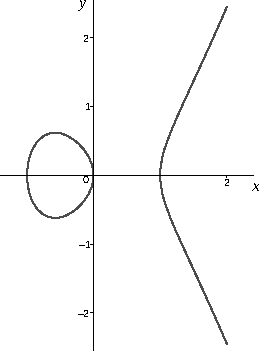
\includegraphics[width=.9\linewidth]{Graficos/grafo_curva_eliptica_reales_1.pdf}

                $y^2 = x^3 - x$
            \end{center}

            \column{0.5\textwidth}
            \begin{center}
                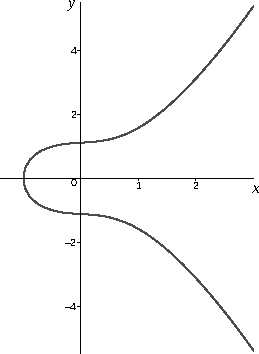
\includegraphics[width=.9\linewidth]{Graficos/grafo_curva_eliptica_reales_2.pdf}

                $y^2 = x^3 + x$
            \end{center}
        \end{columns}
    %\end{exampleblock}
\end{frame}

\begin{frame}{Versión geométrica del método de la cuerda y la tangente}
    %\begin{exampleblock}{}
        \begin{columns}[T,onlytextwidth]
            \column{0.5\textwidth}
            \begin{center}
                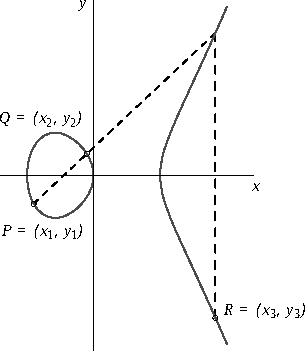
\includegraphics[width=0.8\linewidth]{Graficos/ejemplo_adiccion.pdf}
            \end{center}

            \column{0.5\textwidth}
            \begin{center}
                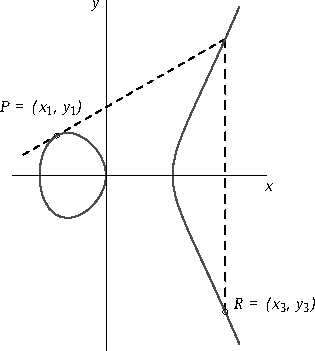
\includegraphics[width=0.8\linewidth]{Graficos/ejemplo_duplicacion.pdf}
            \end{center}
        \end{columns}
    %\end{exampleblock}

    \vfill

    %\metroset{block=fill}
    \uncover<2>{
        \begin{teorema}
            $(E(K), +, \infty)$ es un grupo abeliano.
        \end{teorema}
    }

    \note[item]{ Veamos como dotar de estructura de grupo al conjunto de puntos de una curva elíptica. Para ello definiremos un ley de composición mediante fórmulas algebraicas. Estas formulas están inspiradas en el siguiente método.}
    \note[item]{	Dados dos puntos $P$ y $Q$ , veamos como producir un tercer punto $R$. En primer lugar si $P$ y $Q$ son distintos, los pasos son:
	\begin{enumerate}
		\item Se dibuja una recta $L$ de $P$ a $Q$.
		\item Esta recta intersecta la curva elíptica en un tercer punto.
		\item Tomamos $R$ como la reflexión de este punto sobre el eje-$x$.
	\end{enumerate}
	Si los puntos $P$ y $Q$ son iguales, los pasos son:
	\begin{enumerate}
		\item Se dibuja la línea tangente $L$ a la curva elíptica en $P$.
		\item Esta línea intersecta la curva elíptica en un segundo punto.
		\item Tomamos $R$ como la reflexión de este punto sobre el eje-$x$.
	\end{enumerate}
    }

    \note[item]{Así, este metodo se traduce a formulas algebraicas, se define una operación binaria en el grupo de puntos con dichas formulas  y se prueba... SIGUIENTE!
    }
    \note[item]{ Para cuerpos base con característica 2 o 3, las fórmulas cambian necesariamente. En la memoria se ve la ley de composición para una curva elíptica sobre un cuerpo finito de característica 2.}
\end{frame}

\begin{frame}{Endomorfismos}
    Un \emph{endomorfismo} de $E$ es un homomorfismo $\alpha: \EKca \to \EKca$ dado por funciones racionales $r_1, r_2$
    $$
        \alpha(x, y) = (r_1(x), r_2(x) y).
    $$

	El \emph{grado} de un endomorfismo $\alpha$ es el grado de $r_1$.

    $\alpha$ es \emph{separable} si la derivada $r_1(x)'$ no es idénticamente cero.

    \vfill

    Un ejemplo es el \textit{endomorfismo multiplicación por n}
    $$
        n(P) = n P,\ \forall P \in \EKca.
    $$

    \note[item]{Una parte importante de la teoría de curvas elípticas es la teoría de endomorfismos. Seran una herramienta clave para probar resultados importantes como el teorema de estructura o el teorema de Hase. }

    \note[item]{La definición de endomorfismo es más general ya que tiene que estar dado por funciones racionales en x y en y, pero existe un resultado que afirma basta describir con dos funciones racionales en x.}

    \note[item]{Los dos ultimos tiene sentido para $\alpha \neq 0$. Si alfa es trivial, su grado es 0 y no es separable por definición.}

    \note[item]{El endomorfismo de multiplicación, junto con el endomorfismo de Frobenius que veremos posteriormente son los dos endomorfismos concretos que manejaremos.}
\end{frame}

\begin{frame}{Endomorfismos}

    \begin{proposicion}\label{pp:cardinal del núcleo}
        $\alpha$ es separable $\implies \dega = \left\vert{\ker(\alpha)}\right\vert$.

        $\alpha$ no es separable $\implies
    		\dega > \left\vert{\ker(\alpha)}\right\vert
    	$.
    \end{proposicion}

    \begin{proposicion}\label{pp:sobreyectividad endomorfismos}
        $\alpha \neq 0 \implies \alpha$ es sobreyectiva.
    \end{proposicion}

    \begin{proposicion}\label{pp:endomorfismo multiplicación}
        $n(P)$ es separable $\iff car(K) \nmid n$.
    \end{proposicion}

    \note[item]{alfa un endmorfismo; car(K) la característica del cuerpo K}
    \note[item]{Estos son los principales resultados generales sobre endomorfimos. En la memoria se DEMUESTRAN detalladamente. Serán la base para los siguiente resultados.}
\end{frame}

\begin{frame}{Subgrupos de torsión}
	Un elemento de $\EKca$ cuyo orden es finito se llama \emph{punto de torsión}.

    El \emph{subgrupo de n-torsión} es el subgrupo de $\EKca$ dado por
    $$
        E[n] = \{ P \in \EKca \ | \  n P = \infty \}.
    $$

    \uncover<2>{
        \begin{teorema}\label{th:estructura subgrupos torsión}
            Si $ car(K) \nmid n$, entonces $$E[n] \simeq \mathbb{Z}_n \oplus \mathbb{Z}_n.$$

            Si $car(K) = p > 0$, y $p | n$, entonces $$E[n] \simeq \mathbb{Z}_{n'} \oplus \mathbb{Z}_{n'} \ \textrm{o} \ \simeq \mathbb{Z}_{n} \oplus \mathbb{Z}_{n'}$$
        	donde $n = p^r n'$ con $p \nmid n'$.
        \end{teorema}
    }

    \note[item]{Otra parte importante de la teoría de curvas elípticas son los subgrupos de torsión.}
    \note[item]{Estos conjuntos son subgrupos ya que son los núcleos del endomorfismo multiplicación por $n$}
    \note[item]{Teroma de estructura
    \begin{itemize}
        \item $n$ un entero positivo, $\oplus$ denota la suma directa de grupos, $Z_n$ grupos cíclicos
        \item Se usa <<el teorema de estructura de grupos abelianos finitos>>.
    \end{itemize}
    }

    \note[item]{Antes de pasar a curvas elípticas sobre cuerpos finitos, en la memoria se desarrollan unas cuantas ideas que aquí comentaremos por encima por cuestión de tiempo.
    \begin{itemize}
        \item En primer lugar, se le asocia una matriz a un endomorfismo.
        \item En segundo lugar, se introduce el emparejamiento Weil, un emparejamiento entre los subgrupos de torsión y el grupo de las raíces n-ésimas de las unidades. Este emparejamiento tiene propiedades muy buenas.
        \item Con esta asociación y el emparejamiento, se consigue calcular el grado de una combinación lineal de endomorfimos a partir del grado de los endomorfismos. Esto se usará en el teorema de Hasse.
    \end{itemize}
    }
\end{frame}

\begin{frame}{Curvas elípticas sobre cuerpos finitos}
    Sea $\Fq$ el cuerpo finito de $q$ elementos.

    $E(\Fq)$ es un grupo abeliano \textit{finito}.

    Un ejemplo importante de endomorfismo sobre $E(\Fqca)$ es el \textit{endormofirsmo de Frobenius}
    $$
        \phi_q(x, y) = (x^q, y^q), \quad \phi_q(\infty) = \infty
    $$

    \uncover<2>{
        \begin{proposicion}\label{pp:relacion nucleo y endomorfismo Frobenius}
            Sea $E$ una curva elíptica definida sobre un cuerpo finito $\Fq$ y consideremos el endomorfismo $\phiq^n - 1$ con $n \ge 1$. Entonces
            \begin{enumerate}
                \item $\ker(\phiq^n - 1) = E(\F_{q^n})$.
                \item $\phiq^n - 1$ es separable, por lo que $\left\vert{E(\F_{q^n})}\right\vert = \deg(\phiq^n - 1)$.
            \end{enumerate}
        \end{proposicion}
    }

    % TODO: introducir
    \note[item]{A partir de ahora, se particulariza los resultados vistos a curvas elípticas sobre cuerpos finitos. En la memoria sale:
    \begin{itemize}
        \item La particularización del teorema de estructura.
        \item La definición de supersingularidad y las formulas de adicción para cuerpos finitos de característica 2.
    \end{itemize}}

    \note[item]{El endomorfismo de Frobenius es la generalización del endomorfismo de Frobenius sobre
cuerpos de caracterítica p. Se prueban numeros resultados sobre el endomorfismo de Frobenius y variantes, pero sin duda la más importante es... SIGUIENTE}

\end{frame}

\begin{frame}{Teorema de Hasse}
    \metroset{block=fill}
    \begin{block}{Teorema de Hasse}
        Sea $E$ una curva elíptica definida sobre un cuerpo finito $\Fq$. Entonces el orden de $E(\Fq)$ verifica
        $$
            |q + 1 - \left\vert{E(\F_{q})}\right\vert| \le 2 \sqrt{q}.
        $$
    \end{block}

    \note[itemize]{
    \begin{nota}[comentarios del teorema~\ref{th:teorema de Hasse}]\leavevmode
    	\begin{itemize}
    		\item Como la ecuación de Weierstrass tiene al menos dos soluciones para todo $x \in \Fq$, una primera acotación del orden de $E(\Fq)$ es  $\left\vert{E(\F_{q})}\right\vert \in [1, 2 q + 1]$. El teorema de Hasse proporciona cotas más optimas:
    		$$
    		\left\vert{E(\F_{q})}\right\vert \in [q + 1 - 2 \sqrt{q}, \ q + 1 + 2 \sqrt{q}].
    		$$
    		Como $2\sqrt{q}$ es pequeño respecto a $q$, $E(\Fq) \approx q$.
    		\item Tres resultados fueron clave para la demostración:
    			\begin{itemize}
    				\item La identificación de $E(\Fq)$ con el núcleo de $\phiq - 1$.
    				\item La igualdad entre el orden del núcleo y el grado de $\phiq - 1$ gracias a la separabilidad de $\phiq - 1$.
    				\item El emparejamiento Weil, especialmente la parte (6) del teorema~\ref{pp:endomorfismo Weil} y su consecuencia~\ref{pp:relacion nucleo y endomorfismo Frobenius}.
    			\end{itemize}
    	\end{itemize}
    \end{nota}
    }
\end{frame}

\section{Criptografía con curvas elípticas}

\begin{frame}{RSA vs ECC}
\end{frame}

\begin{frame}{El problema del logaritmo discreto sobre curvas elípticas}
\end{frame}

\begin{frame}{Parámetros de dominio y pareja de llaves}
\end{frame}

\begin{frame}{ECDH}
\end{frame}


\section{ccepy}

\begin{frame}{Criptografía con Curvas Elípticas con Python}
    \begin{center}
        
\includegraphics[scale=0.5]{Graficos/python.png}
    \end{center}

    ccepy es una biblioteca escrita en python 3 para operar con el grupo de puntos de una curva elíptica y trabajar con protocolos criptográficos basados en curvas elípticas.

    \note[item]{El principal motivo para implementar un programa y no utilizar
uno ya existente ha sido para aplicar los conceptos aprendidos en el
desarrollo matemático e implementar los algoritmos estudiados en
los apartados 4.1 y 4.2 del desarrollo informático. Sin embargo, y no
menos importante, otro motivo era crear un programa libre y gratuito,
fácil de entender y extender y con una documentación extensa en
español.

A diferencia de grandes soluciones como Magma o Sage, ccepy es
framework minimalista, es decir, provee un conjunto de funcionalidades
imprescindibles para cualquiera que desee trabajar con curvas
elípticas y a partir de dichas funcionalidades es muy fácil añadir nuevas
mejoras. Además, dichas funcionalidades se han implementado
siguiendo un diseño lo más simple posible, de tal forma que entender
el programa en su totalidad requiere un esfuerzo mínimo comparado
con otros software.
}
\end{frame}

\begin{frame}{Herramientas}
    \begin{itemize}
        \item Sphinx
        \item Hypothesis
        \item Google Style Guide
        \item Git
    \end{itemize}

    \note[item]{Para implementar ccepy hemos seguido un diseño orientado a objetos ya que los elementos algebraicos que queremos implementar (enteros módulo un primo, elementos de un cuerpo finito, puntos de una curva elítipca) se pueden manejar muy bien representándolos como objetos y clases}
    \note[item]{sphinx se ha utilizado para realizar la documentación mientras que hypothesis se ha utilizado para realizar pruebas basados en propiedades}
    \note[item]{Se ha utilizado la «Guía de Estilo de Google para Python» para mantener una
convención es la escritura del código}
    \note[item]{Como control de versiones se ha utilizado git. De hecho, tanto el codigo fuente del programa, la documentación, la memoria como la presentación se encuentra en github para que cualquiera pueda leeerlo.}
\end{frame}

\begin{frame}{Módulos}
El software ccepy consta de cuatro módulos principales:
    \begin{itemize}
        \item Aritmética elemental
        \item Cuerpos finitos
        \item Curvas elípticas
        \item Esquemas criptográficos
    \end{itemize}

y uno secundario:
\begin{itemize}
    \item Listado de curvas elípticas.
\end{itemize}

\note[item]{
\begin{itemize}
    \item Este módulo permite operar con enteros módulo un primo p y polinomios cuyos coeficientes sean enteros módulo un primo p.
    \item Este módulo permite operar con elementos de un cuerpos finito de
q elementos, donde q será la potencia de un primo.
    \item Este módulo permite operar con el grupo de puntos de una curva
elíptica.
    \item Este módulo permite trabajar con protocolos criptográficos asimétricos, como el esquema Diffie-Hellman conocido como ECDH o el
algoritmo de firmas digitales conocido como ECDSA.
\end{itemize}

}
\note[item]{Además de un módulo secundario <<Listado de curvas elípticas>>. Este módulo secundario consiste en una lista de parámetros de
dominio obtenidos de los estándares}

\note[item]{Aparte de los algoritmos listados en el desarrolo teórico, se han implementado algoritmos como:
\begin{itemize}
    \item  algoritmo extendido de Euclides para enteros y plinomios
    \item  ver si un polinomio es irreducible
    \item  algoritmo de exponenciación binaria
\end{itemize}}
\end{frame}

% TODO: hacer al final
% \begin{frame}{Pruebas basadas en propiedades}
%     Se han utilizado dos tipos de pruebas para garantizar la correción
% del programa: pruebas unitarias y pruebas basadas en propiedades.
%
%
% \end{frame}

\begin{frame}[plain]
    \hspace*{-11mm}
    % \vspace{3mm}
    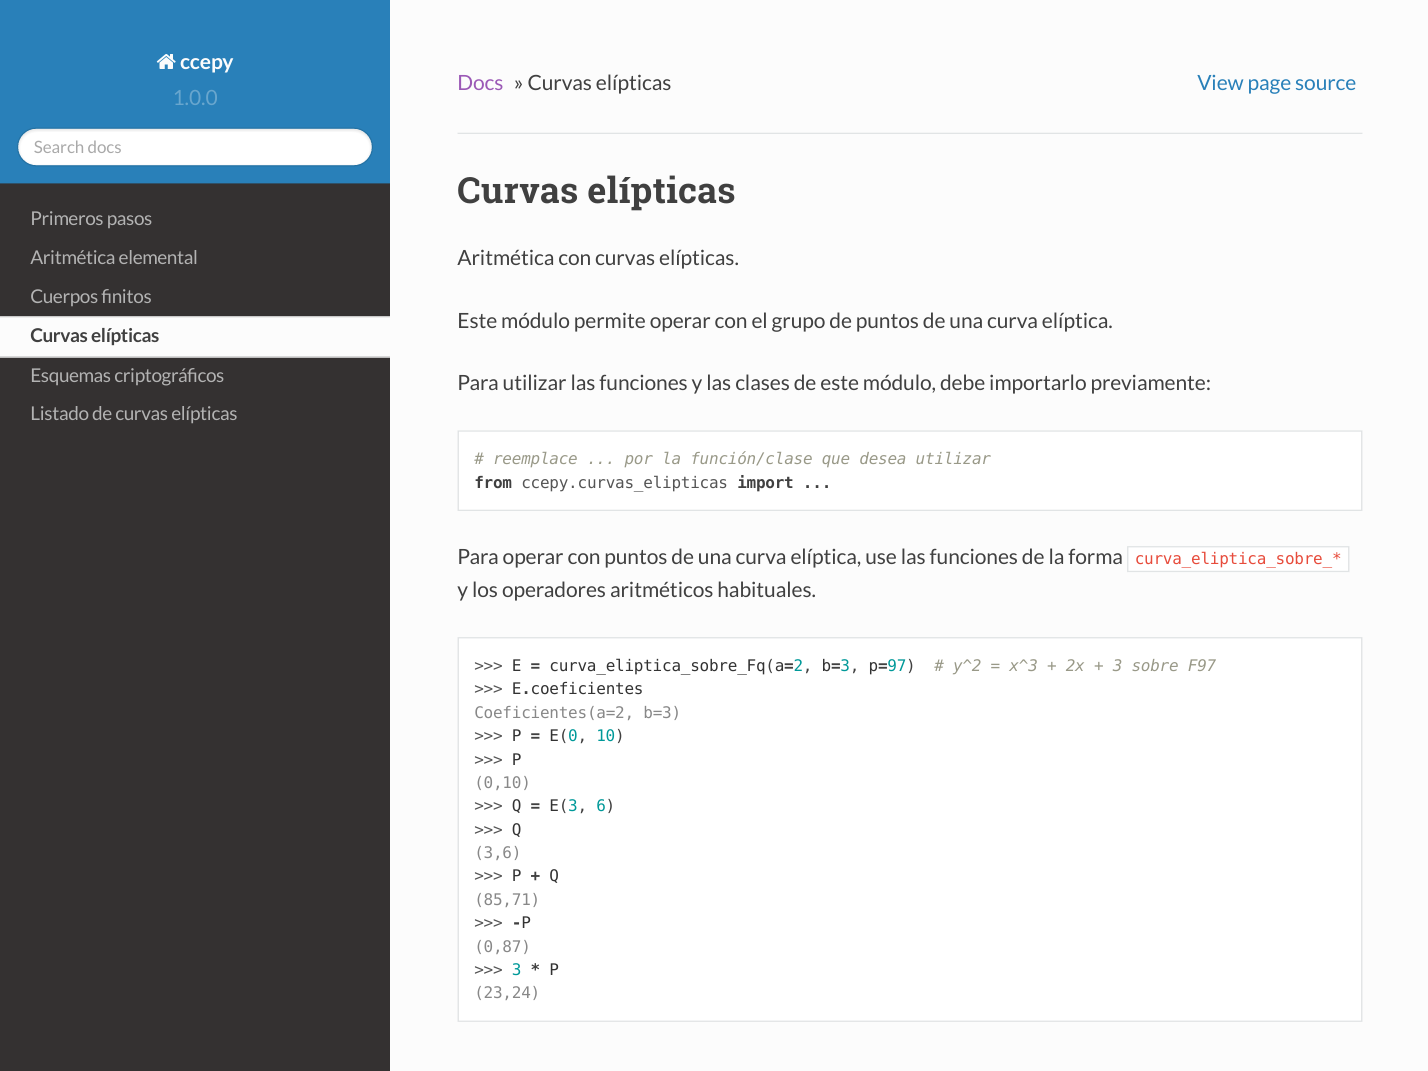
\includegraphics[width=\paperwidth]{Graficos/ejemplo_documentacion}

    \note[item]{ Se ha realizado una documentación, en formato de página web, con cómo instalar y usar ccepy junto con una lista de las funciones, las clases con sus atributos y sus métodos detallados y cada uno con numeros ejemplos de uso}

    \note[item]{ La documentación se ha generado con la biblioteca externa sphinx. El proceso de documentación está detallado en la memoria}
\end{frame}

\begin{frame}[fragile]{Usando ccepy}
    Para instalar la última versión de ccepy:
    \begin{verbatim}
  pip install ccepy
    \end{verbatim}

    Un ejemplo de aritmética de curvas elípticas:
    \begin{verbatim}
  >>> E = curva_eliptica_sobre_Fq(a=2, b=3, p=97)
  >>> E(0, 10) + E(3, 6)
  (85,71)
    \end{verbatim}

    \note[item]{PyPI}
    \note[item]{Por ejemplo, dada la curva elíptica definida por la ecuación y2=x3+2x+3y sobre el cuerpo finito de 97 elementos F97F97, el siguiente trozo de código calcula la suma (0,10)+(3,6)}
\end{frame}

\section{Cifrado de las páginas de la UGR}

\begin{frame}{Introducción a HTTPS}
\end{frame}

\begin{frame}{Páginas web de la UGR vulnerables}
\end{frame}

\end{document}
